%! Author = user
%! Date = 25/01/2021

% Preamble
\documentclass[11pt]{article}

\begin{document}

    \subsection{The Factory Method Pattern}
    \begin{itemize}
        \item Problem: If we program to an Implementation we get locked into a specific type. Our code then needs modification if
        our set of concrete type get extended. When creating object using the "new" operator we are forcing ourselves
        to a concrete implementation. e.g. Duck duck = new MallardDuck();
        \item Often we end up writing code with conditional logic to determine which concrete object to create:
        \begin{lstlisting}[language=C++]
Duck duck
if (picnic) {
    duck = new MallardDuck();
} else if (hunting) {
    duck = new DecoyDuck();
} else if (inBathTub) {
    duck = new MallardDuck();
}
        \end{lstlisting}
        \item Here we make run-time decisions for which class to instantiate. When we see this code we know that when
        requirement changes, and we want to add new types, we need to open up this code and change it. This violates
        the Open/Close Principle.
        \item To solve this problem we look at what varies, the creation, and encapsulate it using a factory pattern.
        \item Three different factory patterns exist
        \begin{enumerate}
            \item The Simple Factory
            \item The Factory Method
            \item The Abstract Factory
        \end{enumerate}
        \subsubsection{The Simple Factory Pattern}
        \item With the Simple Factory pattern, we move the code that's responsible for making a product out of the main
        part of the code and into a separate factory object. The client uses the factory to choose which product to create.\\
        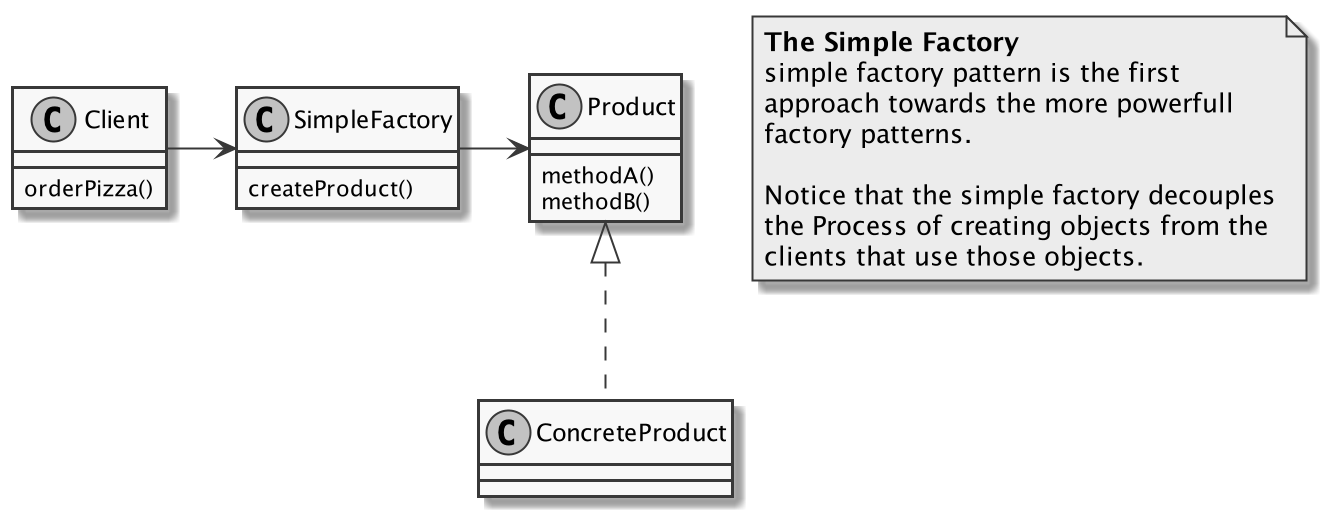
\includegraphics[scale=0.2]{factories/3__simple_factory_pattern}
        \begin{multicols}{2}
            \begin{lstlisting}
class Product {
public:
    virtual void doSomethingWithProduct() = 0;
};

class RegularProduct : public Product {
public:
    void doSomethingWithProduct() override {
        std::cout << "I am regular" << std::endl;
    };
};

class SpecialProduct : public Product {
public:
    void doSomethingWithProduct() override {
        std::cout << "I am special" << std::endl;
    };
};

class ProductFactory {
public:
    std::unique_ptr<Product> MakeProduct(std::string type) {
        if (type == "regular") {
            return std::make_unique<RegularProduct>();
        } else if  (type == "special") {
            return std::make_unique<SpecialProduct>();
        }
    }
};

TEST(SimpleFactory, simple) {
    auto factory = ProductFactory();
    std::vector<std::unique_ptr<Product>> products;
    products.emplace_back(factory.MakeProduct("regular"));
    products.emplace_back(factory.MakeProduct("special"));

    for (auto& p : products){
        p->doSomethingWithProduct();
    }
}
            \end{lstlisting}
        \end{multicols}
        \item The simple factory allows us to decouple the process of creating objects from the clients that uses those
        objects. The simple factory code is the only code that referece to the concrete products. All other code refereces
        to the product interface. We can add concrete products whenever we want, without impacting any code, except the factory.
        \subsubsection{The Factory Method Pattern}
        \item In Factory Method we have a Factory class which operates on products we create but leaves the decision about
        which product to make to the Factory subclasses (instead of deciding itself, like Simple Factory).\\
        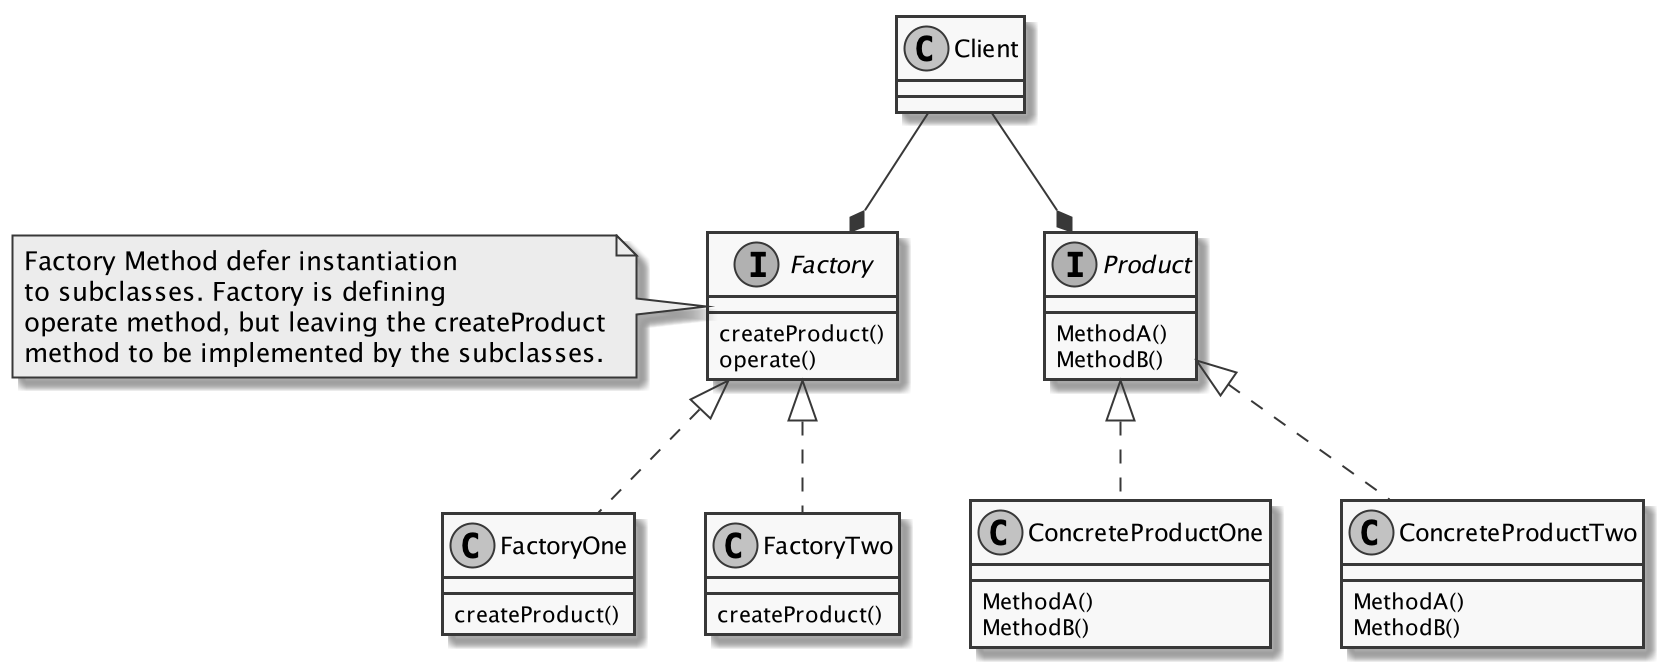
\includegraphics[scale=0.2]{factories/5__factory_method_pattern_general}
        \item Factory Method embodies several design principles, include \textbf{encapsulate what varies}; i.e. factory encapsulate
        the different products that need to get made as well as the code to creates them; \textbf{Program to interace, not implementation};
        i.e. we are programming to product interface in our client code, so we can change the product concrete types without
        having to change the client code. \textbf{Open/Close principle}; i.e. Our factory code is open to new types of products but
        the client is closed for modification. This means we can extend the system with fewer oppertunities for bugs to arise.
        \textbf{Depend on abstractions}. i.e. All code that refers to concrete products is taken completely out of the client, ecapsulated
        into a factory class which makes the client refers only to the pizza interface, not the concrete types of product.
    \end{itemize}

    \subsection{The Abstract Factory}
    Provide an interface for creating families of related or dependent objects without specifying their concrete classes.
    \begin{itemize}
        \item We use the abstract factory pattern whenever we have a system that must be independent of how its products
        are created and represented, and the system is configured with one of multiple families of products.
        \item While Factory Method relies on inheritance, Abstract Factory relies on composition. Object creation is
        implemented in methods exposed in the factory interface.
        \begin{multicols}{2}
            \begin{lstlisting}
// animal.h
class animal {
public:
    virtual ~animal() = default;
    virtual std::string walk() = 0;
    virtual std::string talk() = 0;
};

struct animalItemFactory {
    virtual ~animalItemFactory() = default;
    virtual std::unique_ptr<animal> make() = 0;
};

// ape.h
class ape : public animal {
public:
    std::string walk() override;

    std::string talk() override;
};

struct apeFactory : animalItemFactory {
    std::unique_ptr<animal> make() override {
        return std::make_unique<ape>();
    }
};

// ape.cpp
std::string ape::talk() {
    std::string s = "woegawoega";
    std::cout << s << std::endl;
    return s;
}

std::string ape::walk() {
    std::string s = "with 2 legs";
    std::cout << s << std::endl;
    return s;
}

// dog.h
class dog : public animal {
public:
    std::string walk() override;

    std::string talk() override;
};

struct dogFactory : animalItemFactory {
    std::unique_ptr<animal> make() override {
        return std::make_unique<dog>();
    }
};

// dog.cpp
std::string dog::talk() {
    std::string s = "woof";
    std::cout << s << std::endl;
    return s;
}

std::string dog::walk() {
    std::string s = "with 4 legs";
    std::cout << s << std::endl;
    return s;
}

// animalFactory.h
class animalFactory {
public:
    static constexpr const auto kDog = "dog";
    static constexpr const auto kApe = "ape";

    static std::unique_ptr<animal> make(const std::string &name) {
        return factories_[name]->make();
    }

    static void registers(const std::string &name, std::unique_ptr<animalItemFactory> factory) {
        factories_[name] = std::move(factory);
    }

private:
    static std::map<std::string, std::unique_ptr<animalItemFactory>> factories_;
};

// animalFactory.cpp
static std::map<std::string, std::unique_ptr<animalItemFactory>> init() {
    std::map<std::string, std::unique_ptr<animalItemFactory>> mp;
    mp[animalFactory::kDog] = std::make_unique<dogFactory>();
    mp[animalFactory::kApe] = std::make_unique<apeFactory>();
    return mp;
}

std::map<std::string, std::unique_ptr<animalItemFactory>> animalFactory::factories_ = init();

// client
class zoo {
    zoo() : animal_(animalFactory::make("dog")) {
        animal_->talk();
        animal_->walk();
    }

    std::unique_ptr<animal> animal_;
};
            \end{lstlisting}
        \end{multicols}
    \end{itemize}

    \subsection{The Builder Pattern}
    Separate the construction of a complex object from its representation so that the same construction process can create
    different representations. This pattern is concerend with encapsulating the complexities of how we build an individual object.
    \begin{itemize}
        \item Builder encapsulates the varying details of how a product is assembled, and moving the complexity to
        the concrete builders. The code is easy to write, read and understand. \\
        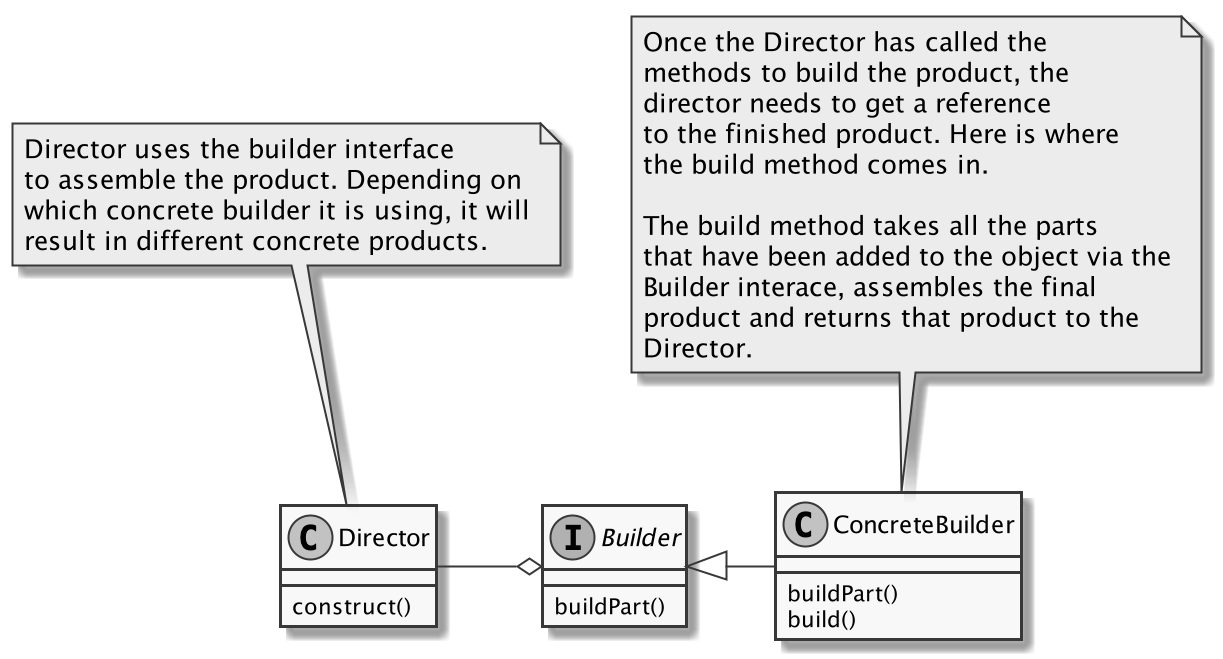
\includegraphics[scale=0.2]{builder/1__builder_pattern}
        \item The intent of the builder pattern is to separate the construction of a complex object from its representation,
        so that the same construction process can be used in different representations of a product.
        \item By creating an interface, we are building in flexibility to the builders we use. It keeps the director and
        client closed for modification.
        \item Builder's lets us vary a product's internal representation (structure of the product)
        \item Using builders gives us fine control over the construction process by splitting the process into steps
        and giving control of that process to the director.
        \item Example: A Car builder.\\
        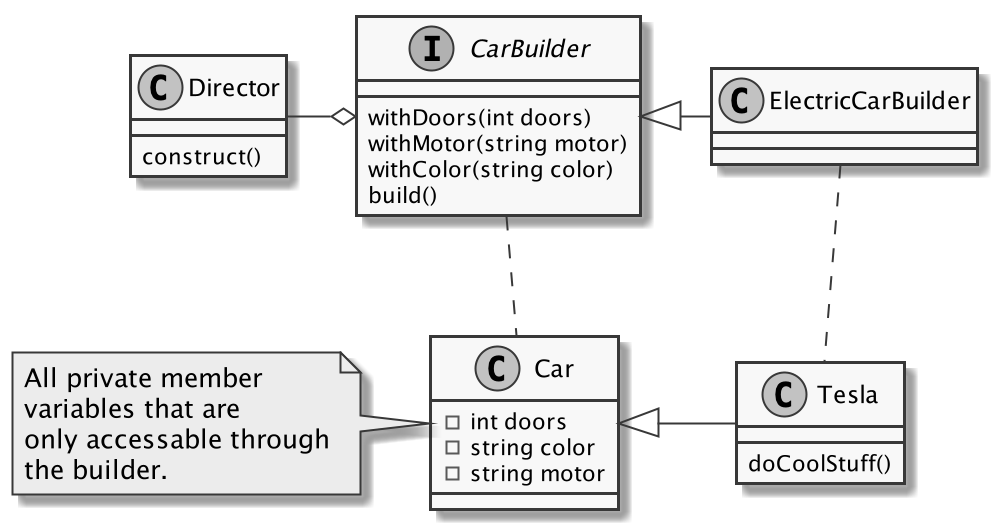
\includegraphics[scale=0.2]{builder/2__builder_pattern_car}
        \begin{multicols}{2}
            \begin{lstlisting}
class CarBuilder;   // forward declare
class ElectricCarBuilder;   // forward declare

class Car {
protected:
    int doors;
    string color;
    string motor;
};

class CarBuilder {
    virtual CarBuilder& withDoors(int doors) = 0;
    virtual CarBuilder& withMotor(string motor) = 0;
    virtual CarBuilder& withColor(string color) = 0;
};

class ElectricCar : public Car {
public:
    static ElectricCarBuilder createBuilder();
    friend ElectricCarBuilder;

    friend std::ostream& operator << (std::ostream &os, const ElectricCar &obj) {
        return os << "doors: " << obj.doors
                  << " color: " << obj.color
                  << " motor: " << obj.motor;
    }
};

class ElectricCarBuilder : CarBuilder {
private:
    typedef ElectricCarBuilder Self;
    ElectricCar c;
public:
    ElectricCar& electric_car;

    ElectricCarBuilder(ElectricCar& e_car) : electric_car(e_car){}
    ElectricCarBuilder() : electric_car(c) {  }

    // setters
    Self& withDoors(int doors) override {
        std::cout << __func__ << std::endl;
        electric_car.doors = doors;
        return *this;
    }
    Self& withMotor(string motor) override {
        std::cout << __func__ << std::endl;
        electric_car.motor = motor;
        return *this;
    }
    Self& withColor(string color) override {
        std::cout << __func__ << std::endl;
        electric_car.color = color;
        return *this;
    }
    ElectricCar build(){
        return c;
    }
};

ElectricCarBuilder ElectricCar::createBuilder() {
    return ElectricCarBuilder();
};

TEST(builder, simple_facet_builder) {
    auto builder = ElectricCar::createBuilder();
    auto e_car = builder
            .withDoors(4)
            .withMotor("Electric")
            .withColor("Red")
            .build();
}
            \end{lstlisting}
        \end{multicols}
    \end{itemize}

    \subsection{The Prototype Pattern}
    Specify the kinds of objects to create using a prototypical instance, and create new objects by copying this prototype.
    \begin{itemize}
        \item We encapsulate the creation of a new object inside an object we call the prototype object. We create new objects
        of the same kind by cloning (copying) that prototype object.
        \item The main benifit is that we separate the client from the details of object creation. We we need flixibility to
        vary the types of objects that we create, we encapsulate what varies by moving the object creating code out of the
        client and into another part of the system. With the prototype pattern we move the creating code into a method
        of the object itself.
        \item Why not factory/new?
            \begin{enumerate}
                \item When we copy an existing object, we get the complex setup for free.
                \item We don't need to know the concrete class of the object that we are creating.
                \item The client is independent of how an object is created.
            \end{enumerate}
        \item We are programming to the interface, not the implementation. So the client doesn't need to know the concrete
        class of the prototype it's using to create new objects, or details of how new objects of that type are created. \\
        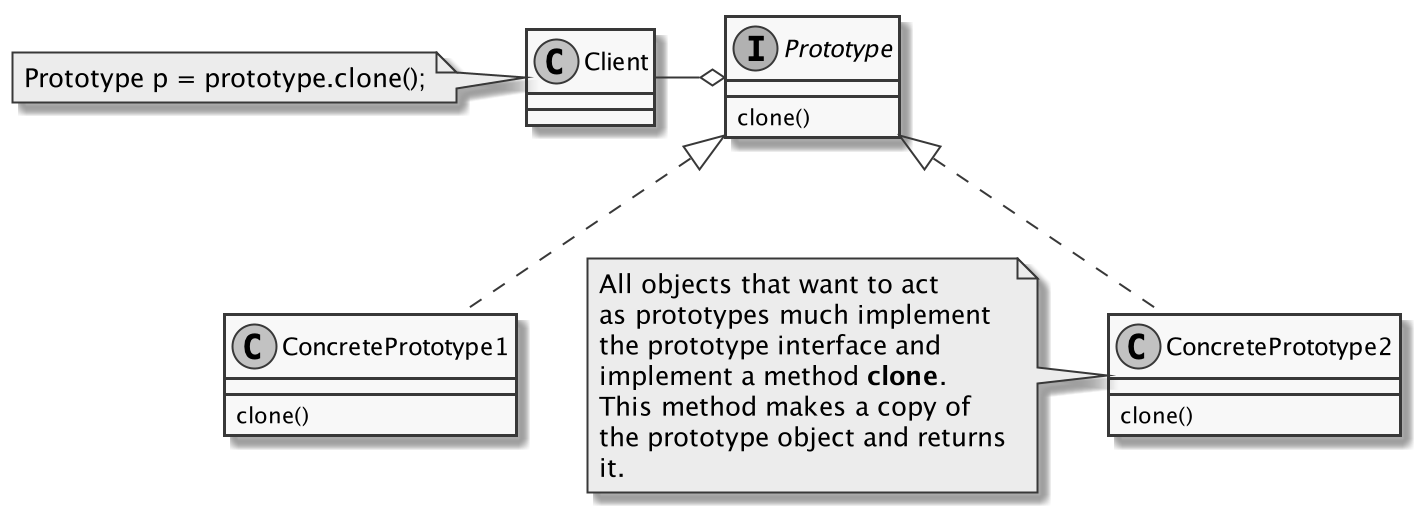
\includegraphics[scale=0.2]{prototype/1__prototype}
        \item Prototype is particularly helpful when we're creating objects that are complex  or expensive to create new.
        We have an existing object we can leverage, so by copying that existing object, we may be albe to create new
        objects more efficiently.
        \item Example: Contact Prototype.
        \begin{multicols}{2}
            \begin{lstlisting}
struct Address {
    string street;
    string city;
    int suite;
};

struct Contact {
    string name;
    Address* work_address;

    Contact(const string& name, Address* const work_address)
            : name(name),
              work_address(new Address(*work_address)) {}

    ~Contact() {
        delete work_address;
    }

    Contact(const Contact& other)
            : name(other.name),
              work_address(new Address(*other.work_address)) {}
};

struct EmployeeFactory {
public:
    // these are the address prototypes
    static Contact main, aux;

    // we clone the prototype by passing the prototype into the copy constructor.
    static unique_ptr<Contact> NewMainOfficeEmployee(string name, int suite) {
        return NewEmployee(name, suite, main);
    }
    static unique_ptr<Contact> NewAuxOfficeEmployee(string name, int suite) {
        return NewEmployee(name, suite, aux);
    }
private:
    static unique_ptr<Contact> NewEmployee (string name, int suite, Contact& proto) {
        auto result = make_unique<Contact>(proto);
        result->name = name;
        result->work_address->suite = suite;
        return result;
    }
};

// these are the contact prototypes
Contact EmployeeFactory::main{"", new Address{"123 EsatDr", "London", 0}};
Contact EmployeeFactory::aux{"", new Address{"123B EsatDr", "London", 0}};

TEST(prototype, factory_prototype) {
    auto john = EmployeeFactory::NewMainOfficeEmployee("John", 100);
    auto jane = EmployeeFactory::NewAuxOfficeEmployee("Jane", 123);

    EXPECT_EQ(jane->work_address->suite, 123);
    EXPECT_EQ(john->work_address->suite, 100);
}
            \end{lstlisting}
        \end{multicols}
    \end{itemize}

    \subsection{The Singleton Pattern}
    Ensure a class only has one instance, and provide a global point of access to it.
    \begin{itemize}
        \item Problem:
        \begin{enumerate}
            \item We need to ensure only one instnace of a class exist.
            \item Instance must be easily accessible to clients.
        \end{enumerate}
        \item Encapsulates the code that is managing a resource. \\
        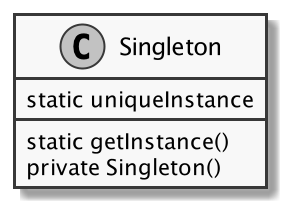
\includegraphics[scale=0.2]{singleton/1__singleton}
        \item The singleton's sole responsibility is to manage a resource.
        \begin{multicols}{2}
            \begin{lstlisting}
class SingletonDatabase {
private:
    SingletonDatabase(){
        // 1. private constructor.
        std::cout << "initializing database" << std::endl;

        std::ifstream ifs("capitals.txt");

        std::string s, s2;
        while (std::getline(ifs, s)) {
            getline(ifs, s2);
            int pop = boost::lexical_cast<int>(s2);
            capitals[s] = pop;
        }

        instance_count++;
    }
    std::map<std::string, int> capitals;

    static SingletonDatabase* instance;

public:
    static int instance_count;
    // 2. delete the copy constructor
    SingletonDatabase(SingletonDatabase const&) = delete;
    // 3. delete the copy assignment
    void operator=(SingletonDatabase const&) = delete;

    static SingletonDatabase& get() {
        // Safe Singleton: this static invocation will only happen once!
        // So thread safe!
        static SingletonDatabase db;
        return db;
    }

    int get_population(const std::string& name) {
        return capitals[name];
    }
};

int SingletonDatabase::instance_count = 0;

TEST(singleton_pattern, naive_approach) {
    auto& db1 = SingletonDatabase::get();
    auto& db2 = SingletonDatabase::get();
    EXPECT_EQ(1, db1.instance_count);
    EXPECT_EQ(1, db2.instance_count);
}
            \end{lstlisting}
        \end{multicols}
    \end{itemize}
\end{document}
